\section{Results} \label{section:results}

In order to reflect how well our models have been trained on different datasets, we report the perplexity for each experiment along with the training steps (from nmt) or epochs (from fairseq). During the training, we store the model parameters of step or epoch which performs best\footnote{Depending on the support of the frameworks, we store the one with best validation BLEU in nmt and the one with best validation loss in fairseq.} on the valid set in a model checkpoint file which is later used to perform decoding on the test set and report the BLEU scores.

\subsection{Training and Validation Perplexities}

% Monument NSpM ppls
\begin{figure}[h]
\centering
\begin{subfigure}{0.3\textwidth}
\includegraphics[width=\textwidth]{../results/monument_600/run1/neural_sparql_machine/ppls.png} 
\caption{NSpM}
\label{fig:monu600 nsm ppl}
\end{subfigure}
\hfill
\begin{subfigure}{0.3\textwidth}
\includegraphics[width=\textwidth]{../results/monument_600/run1/neural_sparql_machine_bahdanau_attention/ppls.png}
\caption{NSpM+Att1}
\label{fig:monu600 nsmbah ppl}
\end{subfigure}
\hfill
\begin{subfigure}{0.3\textwidth}
\includegraphics[width=\textwidth]{../results/monument_600/run1/neural_sparql_machine_luong_attention/ppls.png} 
\caption{NSpM+Att2}
\label{fig:monu600 nsmluo ppl}
\end{subfigure}
\hfill
\begin{subfigure}{0.3\textwidth}
\includegraphics[width=\textwidth]{../results/monument_600/run1/lstm_luong_wmt_en_de/ppls.png}
\caption{LSTM\_Luong}
\label{fig:monu600 lstm ppl}
\end{subfigure}
\hfill
\begin{subfigure}{0.3\textwidth}
\includegraphics[width=\textwidth]{../results/monument_600/run1/wmt16_gnmt_4_layer/ppls.png} 
\caption{GNMT-4}
\label{fig:monu600 gnmt4 ppl}
\end{subfigure}
\hfill
\begin{subfigure}{0.3\textwidth}
\includegraphics[width=\textwidth]{../results/monument_600/run1/wmt16_gnmt_8_layer/ppls.png}
\caption{GNMT-8}
\label{fig:monu600 gnmt8 ppl}
\end{subfigure}
\hfill
\begin{subfigure}{0.3\textwidth}
\includegraphics[width=\textwidth]{../results/monument_600/run2/fconv_wmt_en_de/ppls.png} 
\caption{ConvS2S}
\label{fig:monu600 convs2s ppl}
\end{subfigure}
\hfill
\begin{subfigure}{0.3\textwidth}
\includegraphics[width=\textwidth]{../results/monument_600/run1/transformer_iwslt_de_en/ppls.png}
\caption{Transformer}
\label{fig:monu600 transformer ppl}
\end{subfigure}
\hfill
\caption{Plots of perplexity on the training and validation set of MonumentNSpM for each model}
\label{fig:monu600 ppls}
\end{figure}

Figure \ref{fig:monu600 ppls} shows the graphs of the training and validation perplexity during the training of each model on the MonumentNSpM dataset. Compared to other two monument splits, this dataset has the largest number of training examples, where a full epoch for the fairseq is approximately equivalent to 120 steps for the nmt. After a sufficient number of iterations, all of the models are able to achieve a relatively low perplexity (close to 1) on the training set which means a nearly perfect fitting. On the valid set, all of the models converged at a perplexity between 1 and 1.25, although slight overfittings are observed on two attention-equipped NSpM models as shown in Figure \ref{fig:monu600 nsmbah ppl} and \ref{fig:monu600 nsmluo ppl}. In Figure \ref{fig:monu600 transformer ppl} we noticed an unusual phenomenon that valid perplexity is lower than the training in early epochs.

% Monument80 ppls
\begin{figure}[h]
\centering
\begin{subfigure}{0.3\textwidth}
\includegraphics[width=\textwidth]{../results/monument2_1/run1/neural_sparql_machine/ppls.png} 
\caption{NSpM}
\label{fig:monu1 nsm ppl}
\end{subfigure}
\hfill
\begin{subfigure}{0.3\textwidth}
\includegraphics[width=\textwidth]{../results/monument2_1/run1/neural_sparql_machine_bahdanau_attention/ppls.png}
\caption{NSpM+Att1}
\label{fig:monu1 nsm-bah ppl}
\end{subfigure}
\hfill
\begin{subfigure}{0.3\textwidth}
\includegraphics[width=\textwidth]{../results/monument2_1/run1/neural_sparql_machine_luong_attention/ppls.png} 
\caption{NSpM+Att2}
\label{fig:monu1 nsm-luo ppl}
\end{subfigure}
\hfill
\begin{subfigure}{0.3\textwidth}
\includegraphics[width=\textwidth]{../results/monument2_1/run1/lstm_luong_wmt_en_de/ppls.png}
\caption{LSTM\_Luong}
\label{fig:monu1 lstm ppl}
\end{subfigure}
\hfill
\begin{subfigure}{0.3\textwidth}
\includegraphics[width=\textwidth]{../results/monument2_1/run1/wmt16_gnmt_4_layer/ppls.png} 
\caption{GNMT-4}
\label{fig:monu1 gnmt4 ppl}
\end{subfigure}
\hfill
\begin{subfigure}{0.3\textwidth}
\includegraphics[width=\textwidth]{../results/monument2_1/run1/wmt16_gnmt_8_layer/ppls.png}
\caption{GNMT-8}
\label{fig:monu1 gnmt8 ppl}
\end{subfigure}
\hfill
\begin{subfigure}{0.3\textwidth}
\includegraphics[width=\textwidth]{../results/monument2_1/run2/fconv_wmt_en_de/ppls.png} 
\caption{ConvS2S}
\label{fig:monu1 convs2s ppl}
\end{subfigure}
\hfill
\begin{subfigure}{0.3\textwidth}
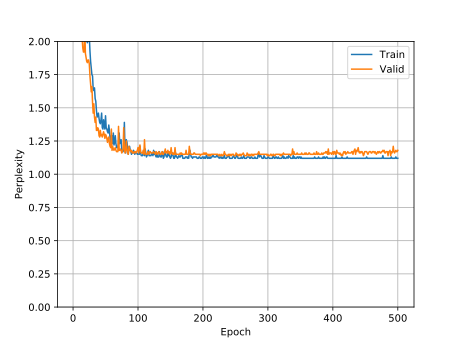
\includegraphics[width=\textwidth]{../results/monument2_1/run1/transformer_iwslt_de_en/ppls.png}
\caption{Transformer}
\label{fig:monu1 transformer ppl}
\end{subfigure}
\hfill
\caption{Plots of perplexity on the training and validation set of Monument80 for each model}
\label{fig:monu1 ppls}
\end{figure}

Figure \ref{fig:monu1 ppls} shows the perplexity graphs on the Monument80 dataset. For this dataset, around 100 steps in the nmt are equivalent to an epoch in the fairseq. The trend of each model is similar with the MonumentNSpM dataset. Given the fact that this dataset contains more valid examples and less training examples than the MonumentNSpM dataset, the valid perplexities are mostly higher but still within the range 1 to 1.5. Slight overfittings are continued to be observed in Figure \ref{fig:monu1 nsm-bah ppl}, \ref{fig:monu1 nsm-luo ppl}, \ref{fig:monu1 gnmt4 ppl}, and \ref{fig:monu1 gnmt8 ppl}.

% Monument50 ppls
\begin{figure}[h]
\centering
\begin{subfigure}{0.3\textwidth}
\includegraphics[width=\textwidth]{../results/monument2_2/run1/neural_sparql_machine/ppls.png} 
\caption{NSpM}
\label{fig:monu2 nsm ppl}
\end{subfigure}
\hfill
\begin{subfigure}{0.3\textwidth}
\includegraphics[width=\textwidth]{../results/monument2_2/run1/neural_sparql_machine_bahdanau_attention/ppls.png}
\caption{NSpM+Att1}
\label{fig:monu2 nsm-bah ppl}
\end{subfigure}
\hfill
\begin{subfigure}{0.3\textwidth}
\includegraphics[width=\textwidth]{../results/monument2_2/run1/neural_sparql_machine_luong_attention/ppls.png} 
\caption{NSpM+Att2}
\label{fig:monu2 nsm-luo ppl}
\end{subfigure}
\hfill
\begin{subfigure}{0.3\textwidth}
\includegraphics[width=\textwidth]{../results/monument2_2/run1/lstm_luong_wmt_en_de/ppls.png}
\caption{LSTM\_Luong}
\label{fig:monu2 lstm ppl}
\end{subfigure}
\hfill
\begin{subfigure}{0.3\textwidth}
\includegraphics[width=\textwidth]{../results/monument2_2/run1/wmt16_gnmt_4_layer/ppls.png} 
\caption{GNMT-4}
\label{fig:monu2 gnmt4 ppl}
\end{subfigure}
\hfill
\begin{subfigure}{0.3\textwidth}
\includegraphics[width=\textwidth]{../results/monument2_2/run1/wmt16_gnmt_8_layer/ppls.png}
\caption{GNMT-8}
\label{fig:monu2 gnmt8 ppl}
\end{subfigure}
\hfill
\begin{subfigure}{0.3\textwidth}
\includegraphics[width=\textwidth]{../results/monument2_2/run2/fconv_wmt_en_de/ppls.png} 
\caption{ConvS2S}
\label{fig:monu2 convs2s ppl}
\end{subfigure}
\hfill
\begin{subfigure}{0.3\textwidth}
\includegraphics[width=\textwidth]{../results/monument2_2/run1/transformer_iwslt_de_en/ppls.png}
\caption{Transformer}
\label{fig:monu2 transformer ppl}
\end{subfigure}
\hfill
\caption{Plots of perplexity on the training and validation set of Monument50 for each model}
\label{fig:monu2 ppls}
\end{figure}

Next, in order to assess the complexity of the monument dataset, we experimented on the Monument50 by further reducing the number of training examples but keeping the same size of the valid set. Here, one epoch is equivalent to 60 steps. The perplexity graphs are shown in Figure \ref{fig:monu2 ppls}. Although the training size is nearly half cut, it appears that the performance on the valid set are not much affected, especially for LSTM\_Luong, ConvS2S, and Transformer which are all implemented in the fairseq. This phenomenon is also reflected on BLEU scores in Table \ref{table:monu50 bleu} and Table \ref{table:monu80 bleu}.  

% LC-QUAD ppls
\begin{figure}[h]
\centering
\begin{subfigure}{0.3\textwidth}
\includegraphics[width=\textwidth]{../results/lc-quad1/run1/neural_sparql_machine/ppls.png} 
\caption{NSpM}
\label{fig:lcquad nsm ppl}
\end{subfigure}
\hfill
\begin{subfigure}{0.3\textwidth}
\includegraphics[width=\textwidth]{../results/lc-quad1/run1/neural_sparql_machine_bahdanau_attention/ppls.png}
\caption{NSpM+Att1}
\label{fig:lcquad nsm-bah ppl}
\end{subfigure}
\hfill
\begin{subfigure}{0.3\textwidth}
\includegraphics[width=\textwidth]{../results/lc-quad1/run1/neural_sparql_machine_luong_attention/ppls.png} 
\caption{NSpM+Att2}
\label{fig:lcquad nsm-luo ppl}
\end{subfigure}
\hfill
\begin{subfigure}{0.3\textwidth}
\includegraphics[width=\textwidth]{../results/lc-quad1/run1/lstm_luong_wmt_en_de/ppls.png}
\caption{LSTM\_Luong}
\label{fig:lcquad lstm ppl}
\end{subfigure}
\hfill
\begin{subfigure}{0.3\textwidth}
\includegraphics[width=\textwidth]{../results/lc-quad1/run1/wmt16_gnmt_4_layer/ppls.png} 
\caption{GNMT-4}
\label{fig:lcquad gnmt4 ppl}
\end{subfigure}
\hfill
\begin{subfigure}{0.3\textwidth}
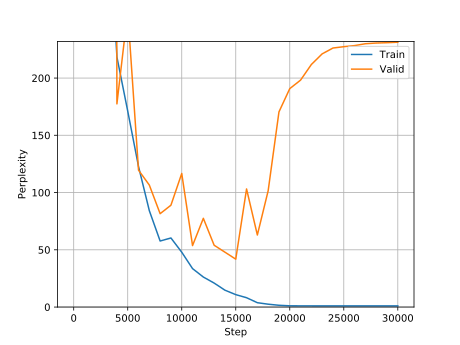
\includegraphics[width=\textwidth]{../results/lc-quad1/run1/wmt16_gnmt_8_layer/ppls.png}
\caption{GNMT-8}
\label{fig:lcquad gnmt8 ppl}
\end{subfigure}
\hfill
\begin{subfigure}{0.3\textwidth}
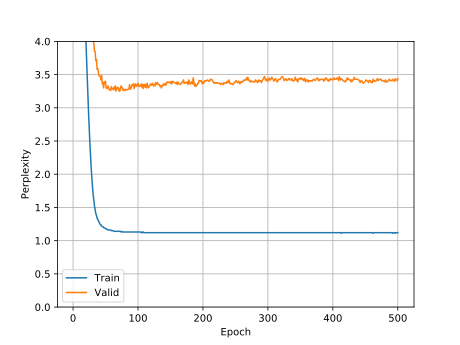
\includegraphics[width=\textwidth]{../results/lc-quad1/run2/fconv_wmt_en_de/ppls.png} 
\caption{ConvS2S}
\label{fig:lcquad convs2s ppl}
\end{subfigure}
\hfill
\begin{subfigure}{0.3\textwidth}
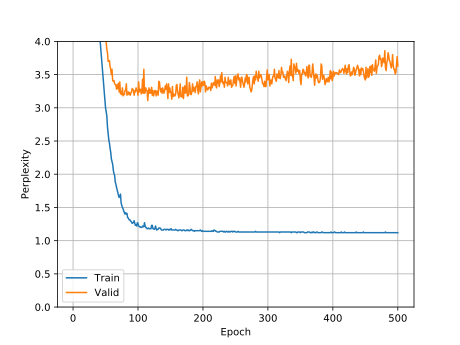
\includegraphics[width=\textwidth]{../results/lc-quad1/run1/transformer_iwslt_de_en/ppls.png}
\caption{Transformer}
\label{fig:lcquad transformer ppl}
\end{subfigure}
\hfill
\caption{Plots of perplexity on the training and validation set of LC-QUAD for each model}
\label{fig:lcquad ppls}
\end{figure}

In the perplexity graphs on the LC-QUAD dataset shown in Figure \ref{fig:lcquad ppls}, we observed a noticeable difference between five models (Figure \ref{fig:lcquad nsm ppl}, \ref{fig:lcquad nsm-bah ppl}, \ref{fig:lcquad nsm-luo ppl}, \ref{fig:lcquad gnmt4 ppl} and \ref{fig:lcquad gnmt8 ppl} have shown serious overfitting at the time of convergence) implemented by the nmt and three models (Figure \ref{fig:lcquad lstm ppl}, \ref{fig:lcquad convs2s ppl} and \ref{fig:lcquad transformer ppl}) implemented by the fairseq. LC-QUAD is much smaller but more complicated compared to other datasets. It only takes 34 steps to finish training an epoch inside the nmt framework. Most of the models have difficulty of providing low perplexity on the valid set, among which GNMT-8 performed the worst and ConvS2S the best. 

%DBNQA ppls
\begin{figure}[h]
\centering
\begin{subfigure}{0.3\textwidth}
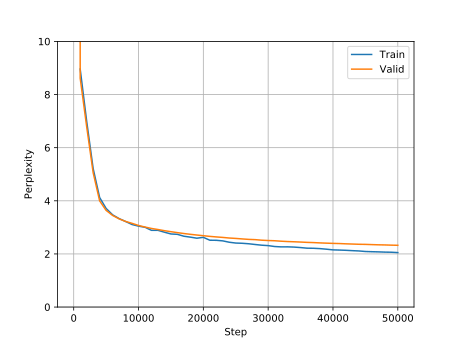
\includegraphics[width=\textwidth]{../results/dbnqa1/run1/neural_sparql_machine/ppls.png} 
\caption{NSpM}
\label{fig:dbnqa nsm ppl}
\end{subfigure}
\hfill
\begin{subfigure}{0.3\textwidth}
\includegraphics[width=\textwidth]{../results/dbnqa1/run1/neural_sparql_machine_bahdanau_attention/ppls.png}
\caption{NSpM+Att1}
\label{fig:dbnqa nsm-bah ppl}
\end{subfigure}
\hfill
\begin{subfigure}{0.3\textwidth}
\includegraphics[width=\textwidth]{../results/dbnqa1/run1/neural_sparql_machine_luong_attention/ppls.png} 
\caption{NSpM+Att2}
\label{fig:dbnqa nsm-luo ppl}
\end{subfigure}
\hfill
\begin{subfigure}{0.3\textwidth}
\includegraphics[width=\textwidth]{../results/dbnqa1/run1/lstm_luong_wmt_en_de/ppls.png}
\caption{LSTM\_Luong}
\label{fig:dbnqa lstm ppl}
\end{subfigure}
\hfill
\begin{subfigure}{0.3\textwidth}
\includegraphics[width=\textwidth]{../results/dbnqa1/run1/wmt16_gnmt_4_layer/ppls.png} 
\caption{GNMT-4}
\label{fig:dbnqa gnmt4 ppl}
\end{subfigure}
\hfill
\begin{subfigure}{0.3\textwidth}
\includegraphics[width=\textwidth]{../results/dbnqa1/run1/wmt16_gnmt_8_layer/ppls.png}
\caption{GNMT-8}
\label{fig:dbnqa gnmt8 ppl}
\end{subfigure}
\hfill
\begin{subfigure}{0.3\textwidth}
\includegraphics[width=\textwidth]{../results/dbnqa1/run1/fconv_wmt_en_de/ppls.png} 
\caption{ConvS2S}
\label{fig:dbnqa convs2s ppl}
\end{subfigure}
\hfill
\begin{subfigure}{0.3\textwidth}
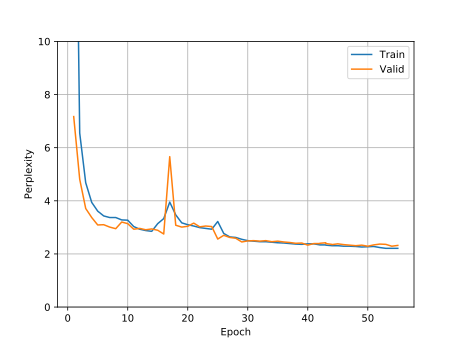
\includegraphics[width=\textwidth]{../results/dbnqa1/run1/transformer_iwslt_de_en/ppls.png}
\caption{Transformer}
\label{fig:dbnqa transformer ppl}
\end{subfigure}
\hfill
\caption{Plots of perplexity on the training and validation set of DBNQA for each model}
\label{fig:dbnqa ppls}
\end{figure}

Finally, Figure \ref{fig:dbnqa ppls} demonstrates the perplexities on the DBNQA dataset. Across all of the models, no evident overfitting is spotted. In a batch size of 128, an epoch of DBNQA takes nearly 5600 training steps. Due to the large size of DBNQA, some models like NSpM and GNMT-8 have shown rather slow or incomplete convergence since the maximum training steps for them (50k and 30k) are just equivalent to a small number (10 and 6) of epochs. Despite that, all of the models have reached a perplexity of at least 2 on the valid set, where NSpM+Att1, NSpM+Att2, and ConvS2S have achieved lower than 2 as shown in Figure \ref{fig:dbnqa nsm-bah ppl}, \ref{fig:dbnqa nsm-luo ppl}, and \ref{fig:dbnqa convs2s ppl}.

\subsection{BLEU Scores}

The BLEU scores of the best checkpoint from each model are stated in Table \ref{table:monu600 bleu}-\ref{table:dbnqa bleu}. In each table, we primarily listed the BLEU scores on the valid and test set as well as the corresponding index of step or epoch of the selected model checkpoint. In order to refer to the state of the checkpoint at that step or epoch, we also reported the perplexities measured on the training and validation set.

\begin{table}[h]
\centering
\caption{BLEU scores and other information of the best checkpoint from each model on MonumentNSpM dataset}
\label{table:monu600 bleu}
\begin{tabular}{c|c|c|c|c|c}
Models & Train ppl & Valid ppl & \textbf{Valid BLEU} & \textbf{Test BLEU} & Step / Epoch \\
\hline
NSpM & 1.00 & 1.09 & 80.43 & 80.28 & Step 29k \\
NSpM+Att1 & 1.01 & 1.16 & 80.36 & 80.58 & Step 14k \\
NSpM+Att2 & 1.01 & 1.14 & 80.88 & 80.03 & Step 9k \\
GNMT-4 & 1.03 & 1.11 & 80.12 & 79.53 & Step 11k \\
GNMT-8 & 1.04 & 1.15 & 79.30 & 79.07 & Step 10k \\
LSTM\_Luong & 1.11 & 1.19 & 92.39 & 91.67 & Epoch 500 \\
ConvS2S & 1.11 & 1.14 & \textbf{98.35} & \textbf{97.12} & Epoch 500 \\
Transformer & 1.13 & 1.09 & 95.25 & 95.31 & Epoch 138 \\
\end{tabular}
\end{table}

In Table \ref{table:monu600 bleu}-\ref{table:monu50 bleu}, we reported the BLEU scores on three splits of the monument dataset. In all of these experiments, ConvS2S performed the best. It is also the case that LSTM\_Luong, ConvS2S, and Transformer outperformed other models by a large margin (about 10-15 BLEUs), most evident on the MonumentNSpM experiments.

\begin{table}[h]
\centering
\caption{BLEU scores and other information of the best checkpoint from each model on Monument80 dataset}
\label{table:monu80 bleu}
\begin{tabular}{c|c|c|c|c|c}
Models & Train ppl & Valid ppl & \textbf{Valid BLEU} & \textbf{Test BLEU} & Step / Epoch \\
\hline
NSpM & 1.00 & 1.21 & 87.55 & 87.03 & Step 44k \\
NSpM+Att1 & 1.00 & 1.44 & 87.82 & 87.34 & Step 44k \\
NSpM+Att2 & 1.00 & 1.44 & 87.99 & 87.37 & Step 34k \\
GNMT-4 & 1.00 & 1.31 & 85.94 & 85.39 & Step 30k \\
GNMT-8 & 1.01 & 1.32 & 84.94 & 84.14 & Step 30k \\
LSTM\_Luong & 1.11 & 1.24 & 96.35 & 96.12 & Epoch 200 \\
ConvS2S & 1.11 & 1.19 & \textbf{96.74} & \textbf{96.47} & Epoch 500 \\
Transformer & 1.12 & 1.14 & 95.16 & 94.87 & Epoch 267 \\
\end{tabular}
\end{table}

\begin{table}[h]
\centering
\caption{BLEU scores and other information of the best checkpoint from each model on Monument50 dataset}
\label{table:monu50 bleu}
\begin{tabular}{c|c|c|c|c|c}
Models & Train ppl & Valid ppl & \textbf{Valid BLEU} & \textbf{Test BLEU} & Step / Epoch \\
\hline
NSpM & 1.00 & 1.29 & 85.19 & 85.54 & Step 50k \\
NSpM+Att1 & 1.00 & 1.60 & 85.98 & 86.17 & Step 50k \\
NSpM+Att2 & 1.00 & 1.62 & 86.60 & 86.52 & Step 50k \\
GNMT-4 & 1.00 & 1.41 & 82.92 & 83.01 & Step 30k \\
GNMT-8 & 1.00 & 1.59 & 80.35 & 80.76 & Step 30k \\
LSTM\_Luong & 1.11 & 1.26 & 94.05 & 94.75 & Epoch 500 \\
ConvS2S & 1.11 & 1.20 & \textbf{96.44} & \textbf{96.62} & Epoch 500 \\
Transformer & 1.14 & 1.17 & 93.80 & 93.92 & Epoch 108 \\
\end{tabular}
\end{table}

\begin{table}[h]
\centering
\caption{BLEU scores and other information of the best checkpoint from each model on LC-QUAD dataset}
\label{table:lc-quad bleu}
\begin{tabular}{c|c|c|c|c|c}
Models & Train ppl & Valid ppl & \textbf{Valid BLEU} & \textbf{Test BLEU} & Step / Epoch \\
\hline
NSpM & 1.00 & 16.46 & 43.91 & 43.50 & Step 20k \\
NSpM+Att1 & 1.00 & 56.23 & 52.68 & 50.13 & Step 40k \\
NSpM+Att2 & 1.00 & 43.20 & 53.03 & 50.86 & Step 41k \\
GNMT-4 & 1.00 & 33.76 & 43.69 & 42.71 & Step 9k \\
GNMT-8 & 1.01 & 229.96 & 44.32 & 43.91 & Step 27k \\
LSTM\_Luong & 1.12 & 4.92 & 52.43 & 51.06 & Epoch 218 \\
ConvS2S & 1.14 & 3.25 & \textbf{61.89} & \textbf{59.54} & Epoch 71 \\
Transformer & 1.16 & 3.15 & 58.99 & 57.43 & Epoch 163 \\
\end{tabular}
\end{table}

Table \ref{table:lc-quad bleu} shows the performance of each model on the LC-QUAD dataset. The models all achieved relatively lower BLEU scores on this dataset as well as higher perplexities compared to other datasets. Another thing to notice is that the best checkpoints selected here are all from the middle stages of the training, which correlates with the potential overfittings exhibited in Figure \ref{fig:lcquad ppls}.

Table \ref{table:dbnqa bleu} displays the BLEU results on the DBNQA dataset. The ConvS2S model outperformed the NSpM model by around 30 BLEU points here, which is the largest model performance difference across all the datasets. It is also worth mentioning that the scores of the Transformer model declined to the third worst and the results of the NSpM with attentions raised to the second best in this dataset, which is usually the opposite in other datasets.

\begin{table}[h]
\centering
\caption{BLEU scores and other information of the best checkpoint from each model on DBNQA dataset}
\label{table:dbnqa bleu}
\begin{tabular}{c|c|c|c|c|c}
Models & Train ppl & Valid ppl & \textbf{Valid BLEU} & \textbf{Test BLEU} & Step / Epoch \\
\hline
NSpM & 2.05 & 2.32 & 65.89 & 65.92 & Step 50k \\
NSpM+Att1 & 1.07 & 1.42 & 89.87 & 89.87 & Step 50k \\
NSpM+Att2 & 1.05 & 1.37 & 91.51 & 91.50 & Step 50k \\
GNMT-4 & 1.74 & 2.24 & 69.65 & 69.61 & Step 30k \\
GNMT-8 & 2.13 & 2.43 & 68.43 & 68.41 & Step 30k \\
LSTM\_Luong & 1.90 & 2.15 & 77.64 & 77.67 & Epoch 55 \\
ConvS2S & 1.12 & 1.25 & \textbf{96.05} & \textbf{96.07} & Epoch 54 \\
Transformer & 2.21 & 3.34 & 68.68 & 68.82 & Epoch 53 \\
\end{tabular}
\end{table}

\section{Discussion} \label{section:discussion}







